\documentclass[conference]{IEEEtran}
\IEEEoverridecommandlockouts
% The preceding line is only needed to identify funding in the first footnote. If that is unneeded, please comment it out.
\usepackage{cite}
\usepackage{amsmath,amssymb,amsfonts}
\usepackage{algorithmic}
\usepackage{graphicx}
\usepackage{textcomp}
\usepackage{xcolor}
\usepackage{dblfloatfix}
\usepackage{hyperref}
\usepackage{minted}
\def\BibTeX{{\rm B\kern-.05em{\sc i\kern-.025em b}\kern-.08em
    T\kern-.1667em\lower.7ex\hbox{E}\kern-.125emX}}
\begin{document}

\title{Collaborative Learning\\ \large Una soluzione di reinforcement learning\\ applicata a un nodo router di messaggi\\
{\footnotesize Progetto Machine Learning}
}
\author{\IEEEauthorblockN{Matteo Conti}
\IEEEauthorblockA{\textit{matricola qui}} \\
\and
\IEEEauthorblockN{Daniele La Prova}
\IEEEauthorblockA{\textit{0320429}} \\
\and
\IEEEauthorblockN{Luca Falasca}
\IEEEauthorblockA{\textit{matricola qui}} \\
}

\newcommand{\code}[1]{\texttt{#1}}

\maketitle

\begin{abstract}
%TODO:
\end{abstract}

\section{Introduzione}
%TODO:

\subsection{Contesto}
%TODO:

\subsection{Obiettivi}
%TODO:

\section{Metodologia}
%TODO:

\subsection{Modello}
%TODO:

\subsection{Agente}
%TODO:

\subsubsection{AgentFaçade}
%TODO:

\subsubsection{AgentFactory}
%TODO:

\subsubsection{Decisions}
Lo spazio di decisioni in cui un agente può trovarsi ad operare può estendersi
attraverso
diverse dimensioni, ognuna delle quali rappresenta un parametro che costituisce
tale azione. Ad esempio, nel caso del problema in esame un'azione dell'agente è
rappresentabile da un vettore a tre dimensioni così codificato:
\begin{itemize}
\item Azione[0] = invia o non fare nulla;
\item Azione[1] = preleva pacchetto da coda i, con $i \in [0, \code{num\_queues} - 1]$;
\item Azione[2] = seleziona power source j, $j \in [0, \code{num\_power\_sources} - 1]$.
\end{itemize}
Si noti che non tutte le combinazioni di valori di questi parametri
rappresentino dei punti legali all'interno dello spazio delle azioni.
Ad esempio, se la prima componente è pari a 0 (non fare nulla), allora i valori delle
altre componenti devono essere don't care.

Una soluzione può essere ricorrere a un'enumerazione, ovvero si "schiaccia"
lo spazio delle azioni lungo un'unica dimensione i cui valori sono rappresentati 
dalle sole combinazioni che rappresentano azioni legali. È una soluzione semplice e
immediata, tuttavia comporta alcuni problemi:
\begin{itemize}
    \item la dimensione dello spazio delle azioni aumenta molto velocemente rispetto
    all'aumentare delle opzioni disponibili. Nel caso del problema, avere in generale
    10 code e 2 power sources comporta 20 possibili azioni diverse. Aggiungere una
    sola power source aggiunge altre 10 azioni disponibili all'agente.
    \item come conseguenza del primo problema, l'apprendimento dell'agente può
    rallentare. %TODO: inserire calcolo reward
\end{itemize}
Le decisions sono una possibile soluzione che combina i vantaggi dell'enumerazione
cercando di limitarne gli svantaggi. Il concetto chiave consiste nel delegare la scelta
del valore di ogni componente di un'azione a un agente diverso. In questa maniera,
ogni agente è responsabile di prendere una decisione, e l'insieme di decisioni compone
l'azione da intraprendere. 

Talvolta può accadere che alcune decisioni vadano intraprese solo se le decisioni prese
precedentemente lo consentono. Ad esempio, se una decisione ha dato come esito
"non fare nulla", non ha senso che si interroghino gli agenti responsabili
della decisione su quale coda e quale power source usare. Per coprire questo aspetto,
gli agenti che prendono le decisioni sono organizzati in un albero, detto appunto
albero delle decisioni. Il nodo root contiene un riferimento all'agente che prende
la decisione iniziale, che dovrebbe essere di alto livello.
A questo punto possono verificarsi due casi:
\begin{itemize}
    \item Il nodo root è una foglia: Nell'albero esiste solo il nodo root. questo
    è il caso banale in cui l'albero di decisione regredisce a un singolo agente.
    La decisione corrisponde al valore ritornato dall'agente, che dunque è anche
    l'azione da intraprendere.
    \item Il nodo root ha figli: La root dispone di più scelte per la decisione.
    Ad ogni scelta corrisponde un nodo figlio, a cui verrà delegata la successiva
    decisione. Il nodo root interroga l'agente associato alla scelta selezionata
    dal suo agente, e così via fino a raggiungere una foglia.
\end{itemize}
La sequenza di decisioni
intraprese dagli agenti rappresenta un cammino dalla root a una foglia dell'albero
delle decisioni, ed è chiamato decision path.
Ogni nodo interrogato registra la sua decisione all'interno del decision path, 
associando alla propria posizione nel path il nome della sua decisione e il suo
valore. Un esempio è visibile in \autoref{fig:decisions}.

Ogni nodo dell'albero delle decisioni è un Consultant. Un Consultant si occupa
delle seguenti responsabilità:
\begin{itemize}
    \item mantiene un riferimento all'agente che prende la decisione;
    \item Mantiene una lista di consultant figli, ognuno dei quali corrisponde
    a una possibile scelta che il suo agente può prendere;
    \item espone un metodo \code{get\_decisions()}, che prende in input
    lo stato e un decision path (possibilmente vuoto) e aggiunge il suo contributo
    al decision path interrogando il suo agente;
    \item espone un metodo \code{train()}, che prende in input un'Esperienza,
    ovvero una tripla
    decision path, stato, reward e addestra il suo agente e quello dei nodi
    figli che fanno parte del decision path.
\end{itemize}
Lo stato e l'esperienza presi in input da un Consultant sono a loro volta
propagati ai consultant figli che fanno parte del decision path. Inoltre,
ogni Consultant può raffinare lo stato e l'esperienza presi in input dal padre
se vengono specificate delle implementazioni per i metodi \code{deduce\_consultant\_state()}
e \code{deduce\_consultant\_experience()}. Tuttavia, tali deduzioni non sono propagate ai figli
per impedire perdite di informazioni. 

Le caratteristiche delle decisions descritte finora comportano
le seguenti implicazioni:
\begin{itemize}
    \item Tutti gli agenti dei Consultant di uno stesso decision path condividono
    lo stesso stato osservato dalla root, oppure ne osservano una deduzione.
    Per esempio, un consultant potrebbe scartare alcuni parametri dello stato
    poiché non rilevanti per la decisione che deve prendere;
    \item Tutti gli agenti dei Consultant di uno stesso decision path condividono
    la stessa esperienza della root al momento del training, oppure ne osservano
    una deduzione. Ad esempio, un consultant potrebbe
    usare come reward un valore derivato da quello osservato dalla root;
    \item Agenti che non fanno parte di un decision path non sono interrogati al momento
    della richiesta delle decisioni per quel path e non partecipano al training corrispondente.
    Questo vuol dire che tali agenti osserveranno solo gli stati che implicano una loro
    partecipazione nel decision path e rewards che sono frutto di essa;
    \item L'addestramento dei consultant di un decision path può essere fatto in parallelo;
    \item Consultant in profondità nell'albero delle decisioni potrebbero riceve molte meno
    esperienze, a seconda che i consultant dei livelli superiori abbiano preso decisioni
    che portino a un loro coinvolgimento oppure no. Sebbene ciò possa sembrare che ne rallenti
    l'apprendimento, bisogna considerare che tali consultant dispongono di uno spazio delle azioni
    molto più ridotto rispetto a quello di un singolo, monolitico agente che deve orientarsi
    in uno spazio delle azioni che enumera tutte le possibili combinazioni legali di valori
    delle componenti delle azioni. Inoltre, se non ricevono esperienze vuol dire che
    non vengono coinvolti così spesso nella costruzione di un decision path. In sostanza,
    un consultant in profondità nell'albero delle decisioni riceve meno esperienze, ma
    ne necessita di meno affinché l'apprendimento converga.
\end{itemize}

In sostanza, l'obbiettivo del framework delle decisions è quello di poter costruire un albero
delle decisioni dalla cui collaborazione dei consultant emerga un comportamento
equivalente a quello di un agente monolitico basato su un'enumerazione dello spazio
delle azioni, senza dover esserne vincolati dagli svantaggi. Da questa idea
viene il nome di collaborative learning.

\subsection{Simulazione}
%TODO:

\subsubsection{Nodo}
%TODO:

\subsubsection{Nodo - Controller}
%TODO:

\subsubsection{Nodo - Agent Client}
%TODO:

\subsubsection{Nodo - Queue}
%TODO:

\subsubsection{SrcNode}
%TODO:

\subsubsection{Network}
%TODO:


\section{Risultati}
%TODO:

\subsection{Condizioni}

% TODO: una subsection per ogni scenario

\section{Conclusioni}
%TODO:

\subsection{What we have learned?}
%TODO:

\subsection{What we could improve?}
%TODO:

\begin{figure*}
    \centering
    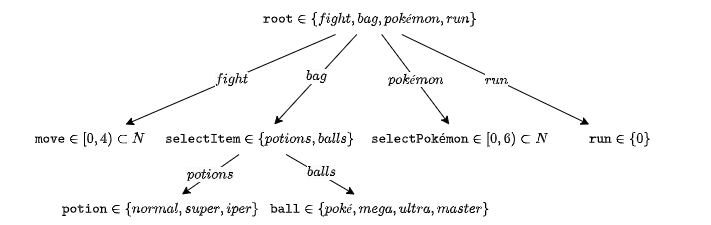
\includegraphics[width=\textwidth]{figs/decisions.drawio.png}
    \caption{Esempio di albero delle decisioni, usando come esempio il combattimento
    nel gioco dei Pokémon. Un esempio di decision path:\\ \code{\{root: bag, select\_item: potions, potion: iper\}}}
    \label{fig:decisions}
\end{figure*}

\end{document}